\chapter{Deep Learning}

\section{Deep Learning}

The Deep Learning framework includes many different models, such as:
\begin{itemize}
    \item Deep Neural Networks;
    \item Convolutional Neural Networks;
    \item Deep belief Networks;
    \item Recurrent and Recursive Neural Networks.
\end{itemize}
They differ from ``shallow'' models in that they have a big amount of layers.

The core concept at the base of deep learning is increasing the level of abstraction of the data through the use of several layers; for example, an image can be gradually abstracted on each layer, first as a vector of intensity values per pixel, then a set of edges, then regions of a particular shape, and so on. The original complicated mapping is broken down into its simple elements, by gradually calculating simpler mapping at each layer. A series of hidden layers extracts increasingly abstract features from a set of example images. Additionally, these abstract features, once learned by the units, can also be combined together to generalize on examples that were never seen during training.

In general, deeper networks are often able to use less units per layer, thus less free parameters as well and less training data required to achieve a good generalization. Still, many layers may be harder to be trained, so there's a need to improve the techniques we know regarding gradient descent, regularization, and data exploitation.

\subsection{Convolutional Neural Networks}

Convolutional Neural Networks are a specialized kind of neural network for processing data with a known, grid-like topology, such as 2D images. The name ``convolutional'' refers to the mathematical operation called \textbf{convolution}, indicated by an asterisk ($*$). This is an operation of two functions of a real valued argument, defined as follows:
\begin{equation*}
    s(t) = (f * g)(t) \stackrel{def}{=} \int_{-\infty}^{\infty} f(\tau)g(t - \tau) d \tau = \int_{-\infty}^{\infty} f(t - \tau)g(\tau) d\tau \,,
\end{equation*}
The idea behind this operator is that we want to calculate the average of $f$ weighted by another function $g$ moved over time (``sliding''), calculated for a certain $t$. In convolutional network terminology, the first argument (here, $f$) is referred to as the \textbf{input}, and the second argument ($g$) as the \textbf{kernel}. The output is called \textbf{feature map}.

This operator can be applied to neural networks as well. Consider a simple network with one hidden layer:
\begin{figure}[ht]
    \centering
    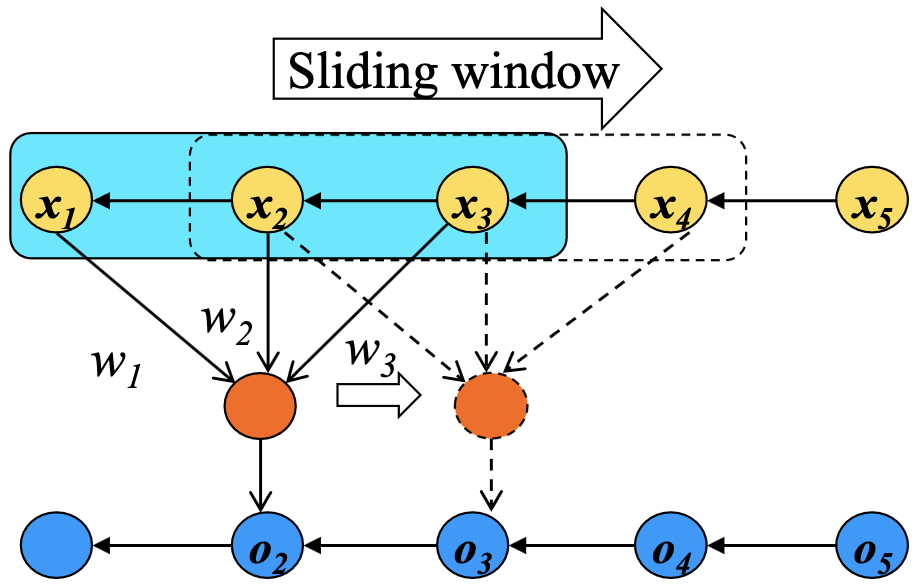
\includegraphics[width=0.45\linewidth]{img/CNN_simple.png}
\end{figure} \\
Here, the output of each node in the hidden layer is calculated as $out_t = \sum_{i=1}^3 w_i x_{t+i-2}$. In other words, the weights assigned to the inputs ``slide'' across the hidden layer. Weights are tuned as usual by learning.

\subsection{2D Convolution}

Discrete convolution can be seen as a multiplication by a matrix, with several entries constrained to be equal to other entries. The convolution over a 2D image $I$ with a kernel $K$ can be expressed as:
\begin{equation*}
    S(i,j) = (I*K)(i,j) = \sum_m \sum_n I(m,n)K(i-m, j-n) \,,
\end{equation*}
or, as expressed by many libraries, as the \textbf{cross-correlation function}:
\begin{equation*}
    S(i,j) = (I*K)(i,j) = \sum_m \sum_n I(i+m,j+n)K(m, n) \,.
\end{equation*}

The example below shows a 2D image with 25 pixels, and a 3x3 kernel (unit local receptive field) with a stride equal to 1 (i.e., the kernel moves across the image 1 pixel at a time; by choosing the stride we choose the size of the feature map). The image also has padding added to its edge.
\begin{figure}[ht]
    \centering
    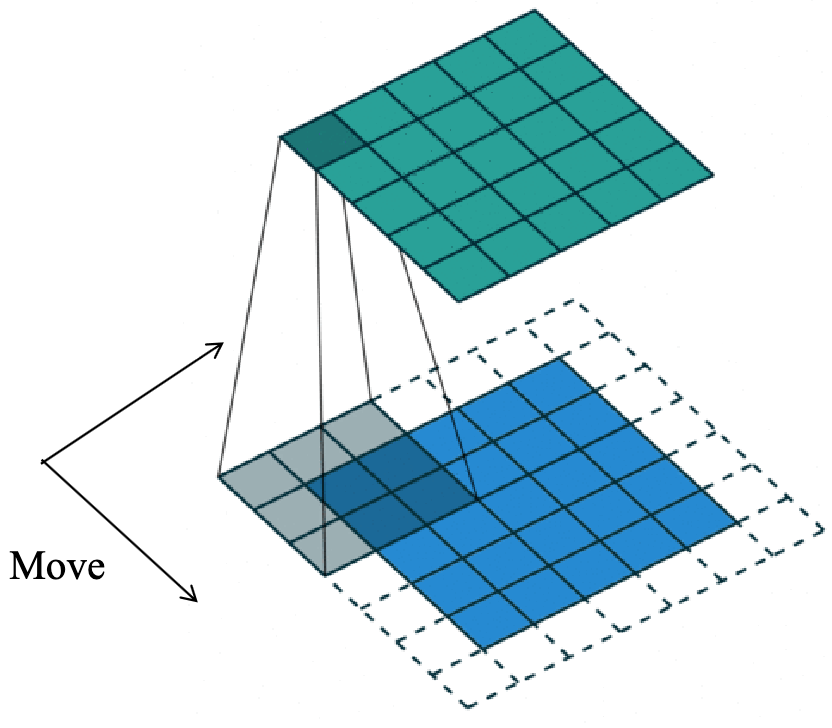
\includegraphics[width=0.6\linewidth]{img/CNN_2D.png} 
\end{figure}

Once the kernel reaches the end of the first ``row'' of pixels, it restarts from the position it started from shifted one pixel below. The full movement of the kernel over the image produces the feature map. The next image better shows the matrix multiplication interpretation of convolution; the image is 4x3 and the kernel is 2x2. The stride is again equal to 1.

\begin{figure}[ht]
    \centering
    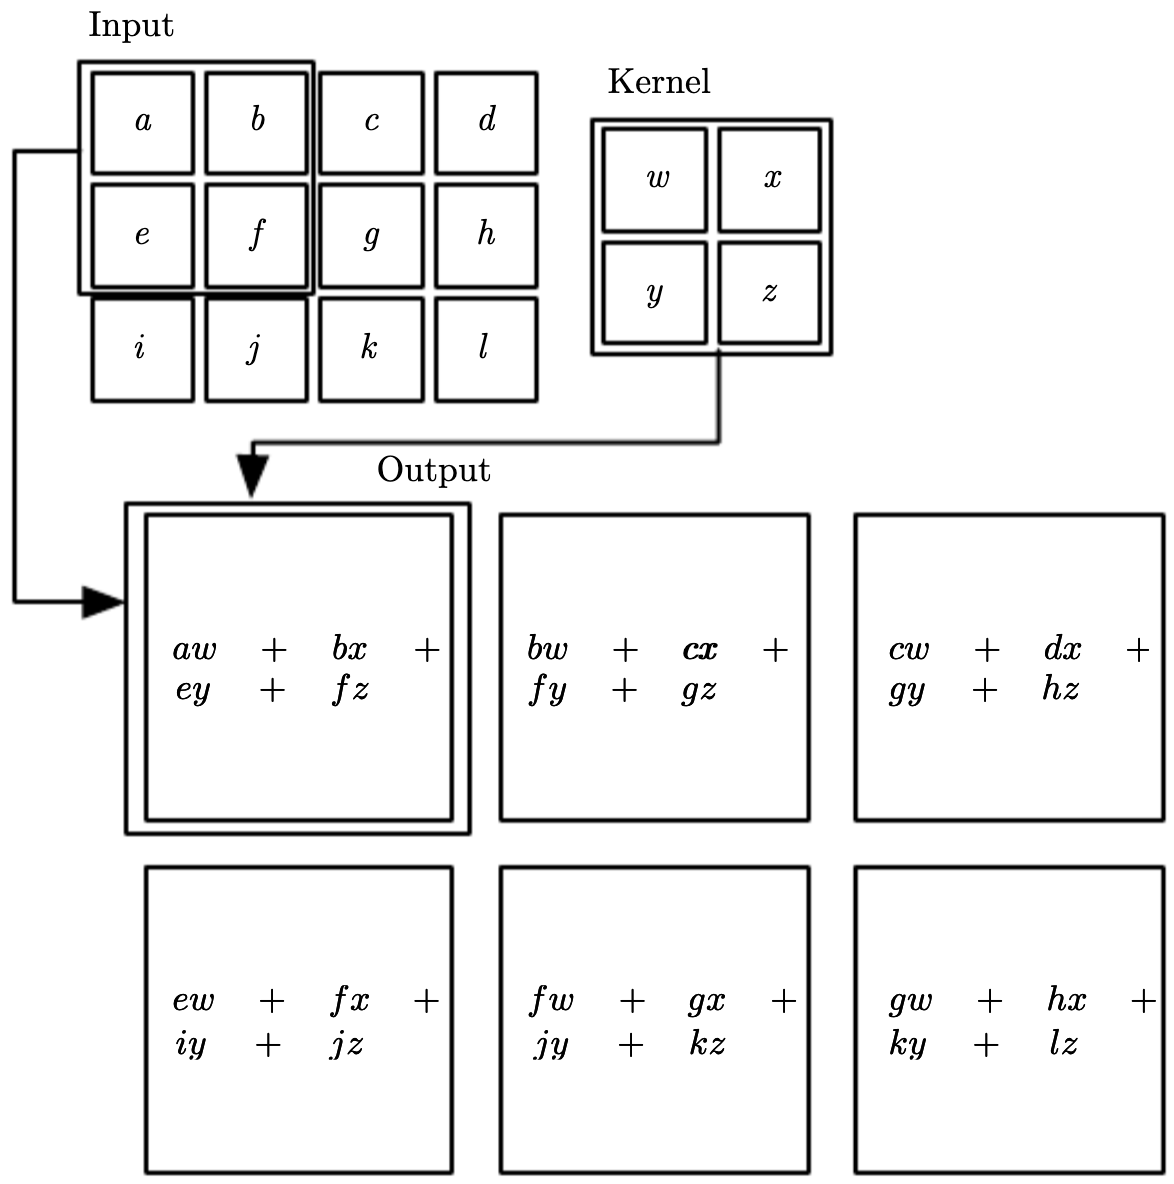
\includegraphics[width=0.5\linewidth]{img/CNN_matrix.png}
\end{figure}
Each unit's weights are a \textbf{filter} trained to detect some specific feature or pattern in the image. Each filter produces the strongest response to a spatially local input pattern, and then the filters obtained by training are applied to the whole (global) image, so that features and patterns can be identified regardless of where they are positioned on the image. \\
The size of the feature map can be reduced via pooling. Some examples of pooling are:
\begin{itemize}
    \item \textbf{Subsampling}, using a stride greater than 1;
    \item \textbf{Average Pooling} (normal or weighted average);
    \item \textbf{Max Pooling} (most common option).
\end{itemize}
This way, instead of producing a value for every single pixel of the original image, we get a smaller set of pixels where each value is obtained by considering the values of neighboring ones (calculating the mean or max value). Pooling also helps to make the representation approximately invariant to small translations of the input, since the mean or max value of a neighborhood of points is unlikely to be affected by a small translation of the pixels in the image.

CNN exploits \textbf{weight sharing}, where the number of connections in the network is kept the same while reducing the number of actual free parameters. The produced sliding window of units is applied over a segment of the input, and reapplied multiple times to produce various layers of feature maps. Training of the weights is usually done via backpropagation. Since these networks tend to be big and deal with large amount of data, many hyperparameters are fixed by experience or by suggestions of experts, since it would be too expensive to run cross-validation.

\subsection{Recurrent Neural Networks}

Up until now, we considered feedforward neural networks. The input is read from the first layer, then traverses a number of hidden layers, and the prediction is finally produced by the output layer. Recurrent neural networks are a different category of architecture, based on the addition of feedback loops to the network topology. These self loops provide the network with dynamical properties, introducing the ability of holding a memory (state) of past computations of the model.

RNNs have been the reference approach for sequence processing, especially for speech and text recognition, processing, and generation. The type of data handled by these models is structured; it is usually an ordered set of sequences of vectors.

The introduction of feedback loops allows the network to hold a memory about past computations. This memory is needed because the output of a certain input depends on previous outputs produced by the same network.
\begin{figure}[ht]
    \centering
    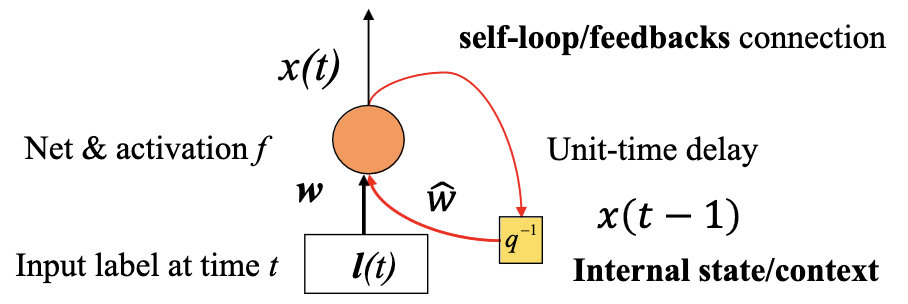
\includegraphics[width=0.5\linewidth]{img/RNN_unit.png}
\end{figure} \\
The output of the node is calculated for a time $t$ recursively, as:
\begin{equation*}
    x(t) = \begin{cases}
            0 & t = 0 \\
            \tau(i(t), x(t-1)) = f(w^Ti(t) + \hat{w}x(t-1) + \theta) & t \geq 0 \\
    \end{cases}
\end{equation*}
Here, $f$ is the activation function of the unit, $i(t)$ is the input label at time $t$, $\hat{w}$ is the recurrent weight (the one that's coming from a feedback), and $\theta$ is the bias. The internal state summarizes the past information, and changes each time the unit produces a new output. The encoding of the past memory is also adaptive. $\tau$ is the state transition function realized by the NN. $x(t)$ here refers only to one state, but it can also include a set of states.

\section{Techniques}

When implementing a deep neural network, there's many technical aspects to consider. As already stated before, the deeper the network, the less units are needed for each layer, and therefore there will be less parameters to train, but some layers may be difficult to train.

\textbf{Batch normalization} is a method that normalizes each batch by calculating each individual batch statistics such as mean and variance for each layer. Each matrix (batch x activation of units) is normalized with mean and variance, shifting the values to zero-mean and unit variance. This technique helps to keep the normalization of the input across all layers of the network. It also achieves a faster learning and higher accuracy for Deep Learning.

\textbf{Dropout} is a method that makes bagging more practical for large neural networks. Dropout trains the ensemble consisting of all sub-networks that can be formed by removing non-output units from an underlying base network. In most modern neural networks, we can effectively remove a unit from a network by multiplying its output value by 0. Then, a minibatch-based learning algorithm is used to train one working sub-network at a time. The sub-network is selected at random, with each binary mask to apply to the original network having a different probability set as an hyperparameter (e.g., 0.8 for input units and 0.5 for hidden units). The sub-networks inevitably share weights, since they're obtained from the same base network; this causes the training of the sub-networks to find good settings for the parameters.

Dropout has a regularization effect as well: it avoids to train all units on all training data and reduces unit interactions. It also reduces variance without affecting bias just like bagging does. It even regularizes singular hidden units to be not just good features, but features that can be good in different contexts (different sub-networks). It can be used for any model that uses distributed representation and SGD training.

\section{Deep Learning for Time Series}

The most commonly used models for time series are:
\begin{itemize}
    \item \textbf{ResNet} (\textbf{residual neural networks}): a deep learning model in which hidden layers learn by receiving both the input of the previous layer and the input to the whole net. Input is forwarded to groups of three convolutional layers each. The final three layers are then connected to a global pooling layer, making the representation of the input smaller and more manageable.
    
    \item \textbf{InceptionTime}: a model made up of inception modules (6 by default), each consisting of convolutions with kernels of different sizes followed by batch normalization, and using the ReLU activation function. The final layer of the net is a regular fully-connected layer with the softmax activation function.
    
    \item \textbf{TapNet}: is made up of three distinct modules; a Random Dimension Permutation which produces groups of randomly selected dimensions, a Multivariate Time Series Encoding, which is 3 sets of convolutional layers followed by batch normalization, and Attentional Prototype Learning, used for unlabeled data.
    
    \item \textbf{CIF} (\textbf{Canonical Interval Forest}): ensemble of time series tree classifiers, built using the 22 Canonical Time Series Features. Each three receives a subsample of the time series and of the features, calculating the features for each interval, and concatenating them to produce a new dataset. The new data is used to build a decision tree.
 
    \item \textbf{ROCKET} (\textbf{Random Convolutional Kernel Transform}): a model that uses a large set of random convolutional kernels to transform the time series. All the parameters of the kernels are randomly generated from fixed distributions, and different kernels may have different length, dilation rate, padding. The transformed data is then used to train a linear classifier (e.g., Logistic Regression or RIdge Regression Classifier). Compared to CNNs, this model is much faster to train since the kernels are not trained, only the final classifier is. Also, in CNNs, dilation increases exponentially with depth, while in ROCKET has a random dilation rate for each kernel. The only hyperparameter of the model is the number of kernels.

    \item \textbf{MINIROCKET}: a faster variant of ROCKET which removes almost all randomness while still yielding good accuracy in classification tasks:
    \begin{itemize}
        \item all kernels have length 9; 
        \item weigths are restricted to two values, $\alpha = -1$ and $\beta = 2$ in the original paper, but can be arbitrarily chosen;
        \item kernels can be chosen out of only 84 possibile ones out of a total of 512 obtainable with length 9;
        \item the bias is drawn from the quantiles of the convolution output for the entire training set and not from a single training example;
        \item each kernel is assigned the same set of dilations, adjusted to the length of the time series;
        \item half of the kernels use padding, the other half don't;
        \item instead of using max pooling, it uses PPV (proportion of positive values) to produce features.
    \end{itemize}
    \item \textbf{COTE, HIVE-COTE, TS-CHIEF}: COTE (which stands for Collective of Transformation-Based Ensemble) combines 35 classifiers over four data representations (similarity measures, shapelet-transform, autocorrelation features, power spectrum). HIVE-COTE (Hierarchical Vote COTE) is an extension of COTE that includes more classifiers and implements a hierarchical voting procedure. TS-CHIEF (Time Series Combination of Heterogeneous and Integrated Embedding Forest) builds a random forest of decision trees whose splitting is based on similarity measures, dictionary representations, and interval-based transformations.

    \item \textbf{MR-SEQL}: data is discretized into sequences (either via SAX or SFA), using a sliding window. The most discriminative windows are extracted using a Sequence Learner algorithm, and the dataset is transformed in terms of presence/absence of subsequences (similarly to shapelet transform). A linear model is then trained on this new representation.
\end{itemize}